\section{Dynamic Aggregation Example and Freshness Scheduling Results}

% In this section we present the experimental methodology and results for \emph{dynamic aggregation} and \emph{freshness scheduling}.

We present a demonstration of \emph{dynamic aggregation} and a describe our methodology and evaluation of
our \emph{freshness scheduling} algorithm.  The first demonstration shows how dynamic aggregation works in a real-world
scenario, as a mobile sensor is moved from one room to another.  The evaluation sets up a realistic scenario and
measures how the algorithm performs in comparison to the standard scheduling approach.

\subsection{Dynamic Aggregation Scenario}
We illustrate dynamic aggregation with a common usage scenario.  It is typical to consider widespread deployment 
of wireless meters when performing an energy audit in a building.  Because such meters are expensive, they are often 
re-used in order to capture a broad sample of energy-consuming items.  We construct an energy auditing application
that provides the user with a mobile mechanism for virtually ``binding'' meters with items, so that accounting of
energy can be done correctly.  Without record the explicit association between the meter and the item is is metering, 
the data stream collected from the meter is meaningless.  Moreover, it is not just meaningless with respect to the item
but meaningless in a broader context of aggregation (i.e. room or floor-level consumption statistics).

For a more specific scenario, imagine there are a number of people in a building,
each owning a number of plug-load appliances and a laptop.  When a person is in a room their laptop
is plugged in and when they leave the room they unplug their laptop and take it with them.  As people come and go
they attached their laptop to a registered meter and the association is automatically recorded in StreamFS.
The meter is constantly reporting readings to StreamFS as well.  

We setup this experiment in a home office environment with two rooms
and set up the room-level nodes as an \emph{aggregation point} for all the meters in the room.  The monitored
2 laptops and 2 lamps and we demonstrate the aggregate power draw of both rooms as we move one of the laptops from
room 1 at tick 7, walk to room 2, and register the laptop in room 2.

%FILL IN WITH REAL GRAPH
\begin{figure}[htb!]
\begin{center}
\subfloat[Room 1 object and aggregate streams.]{%
            \label{fig:dynaggs1room1}
            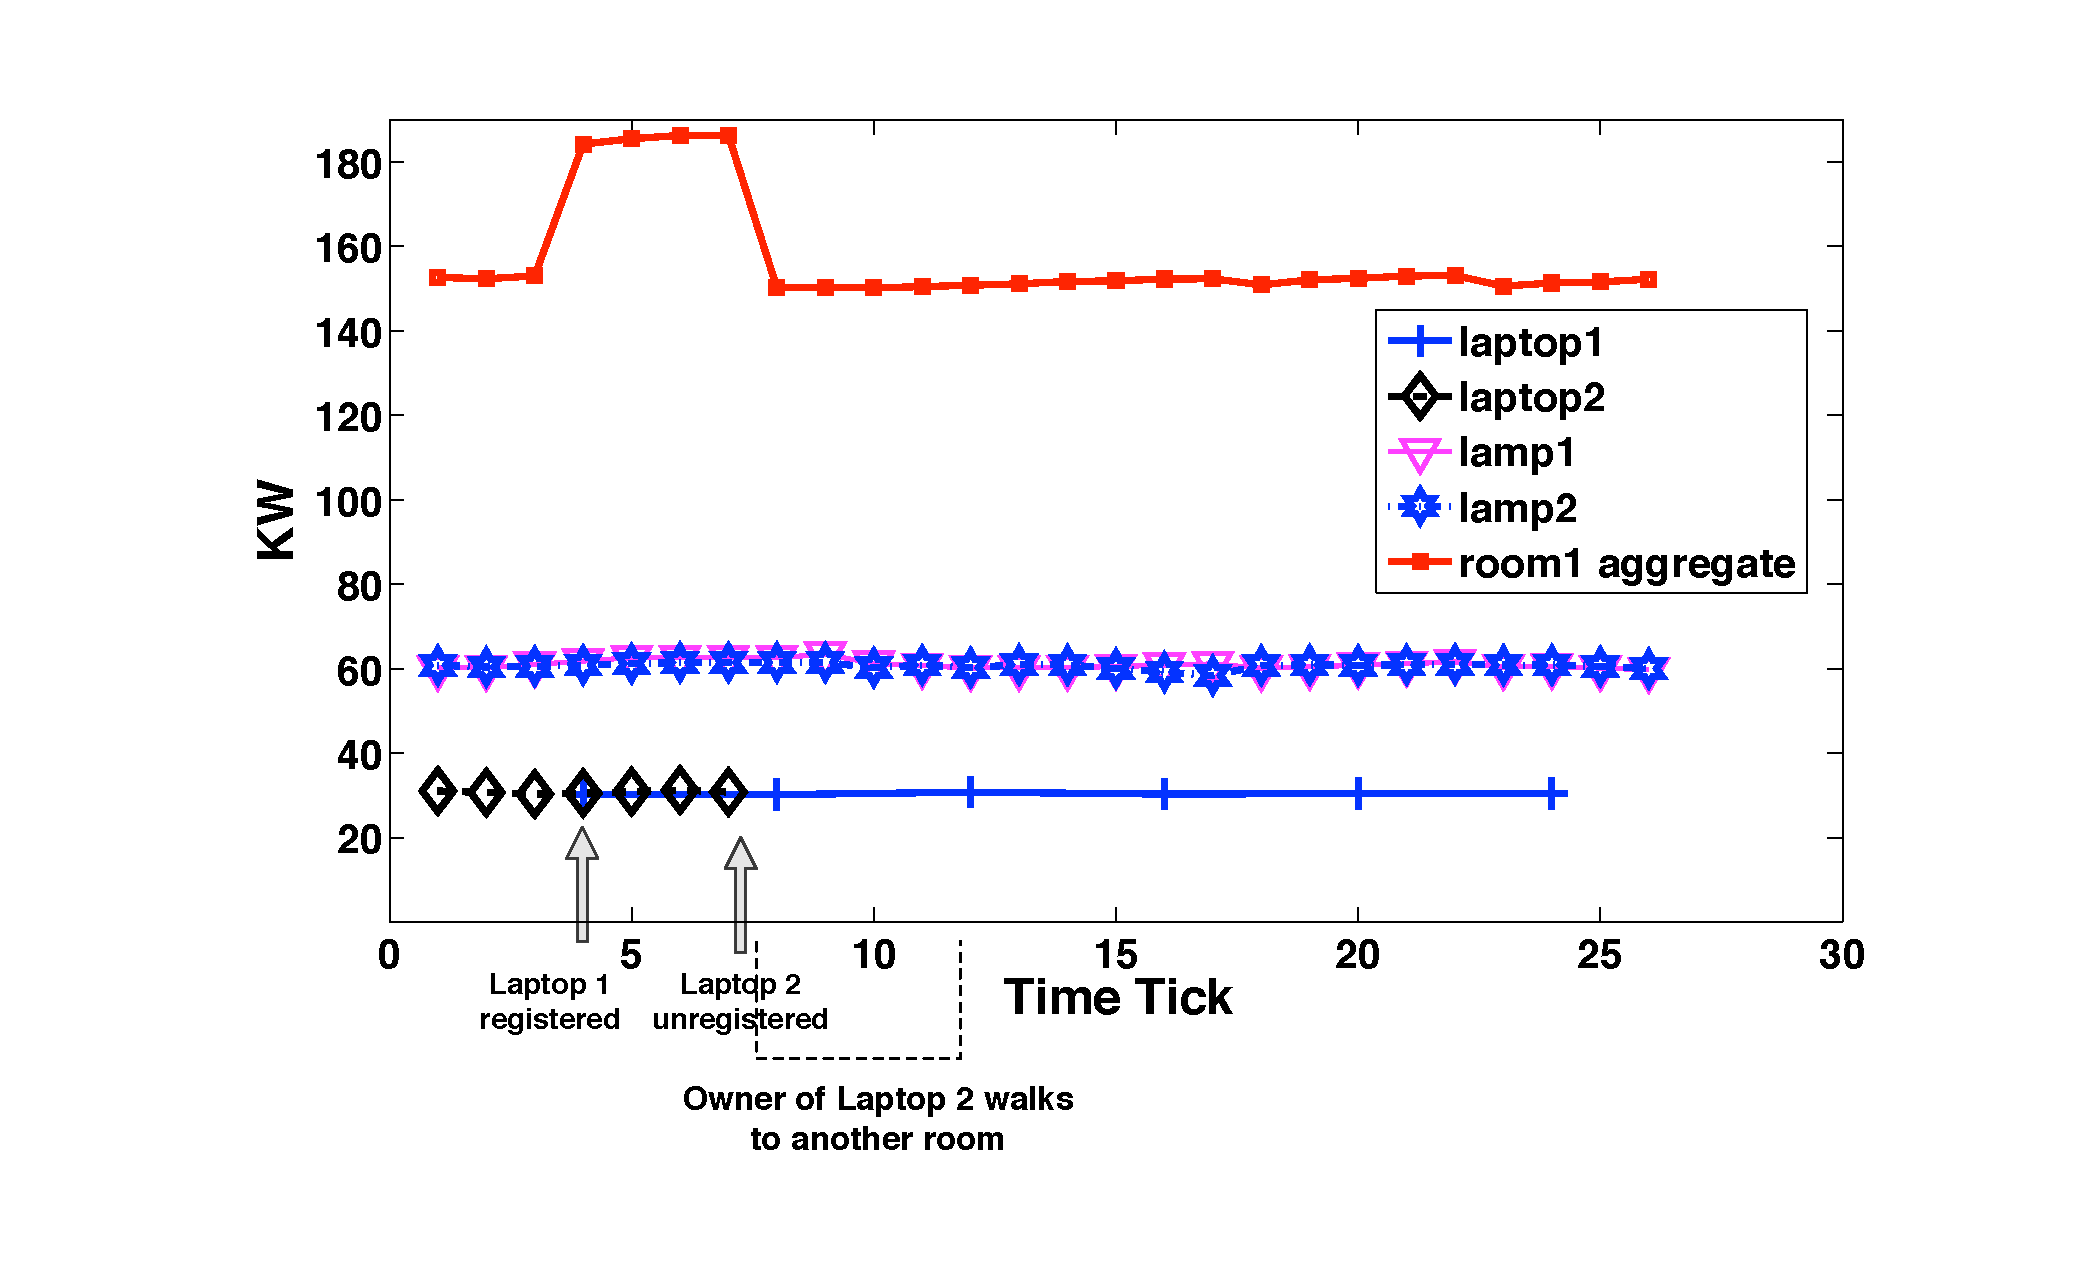
\includegraphics[scale=0.28]{figs/dynagg_scenario1_room1.pdf}
        }
\subfloat[Room 2 aggregate.]{%
            \label{fig:dynaggs1room2}
            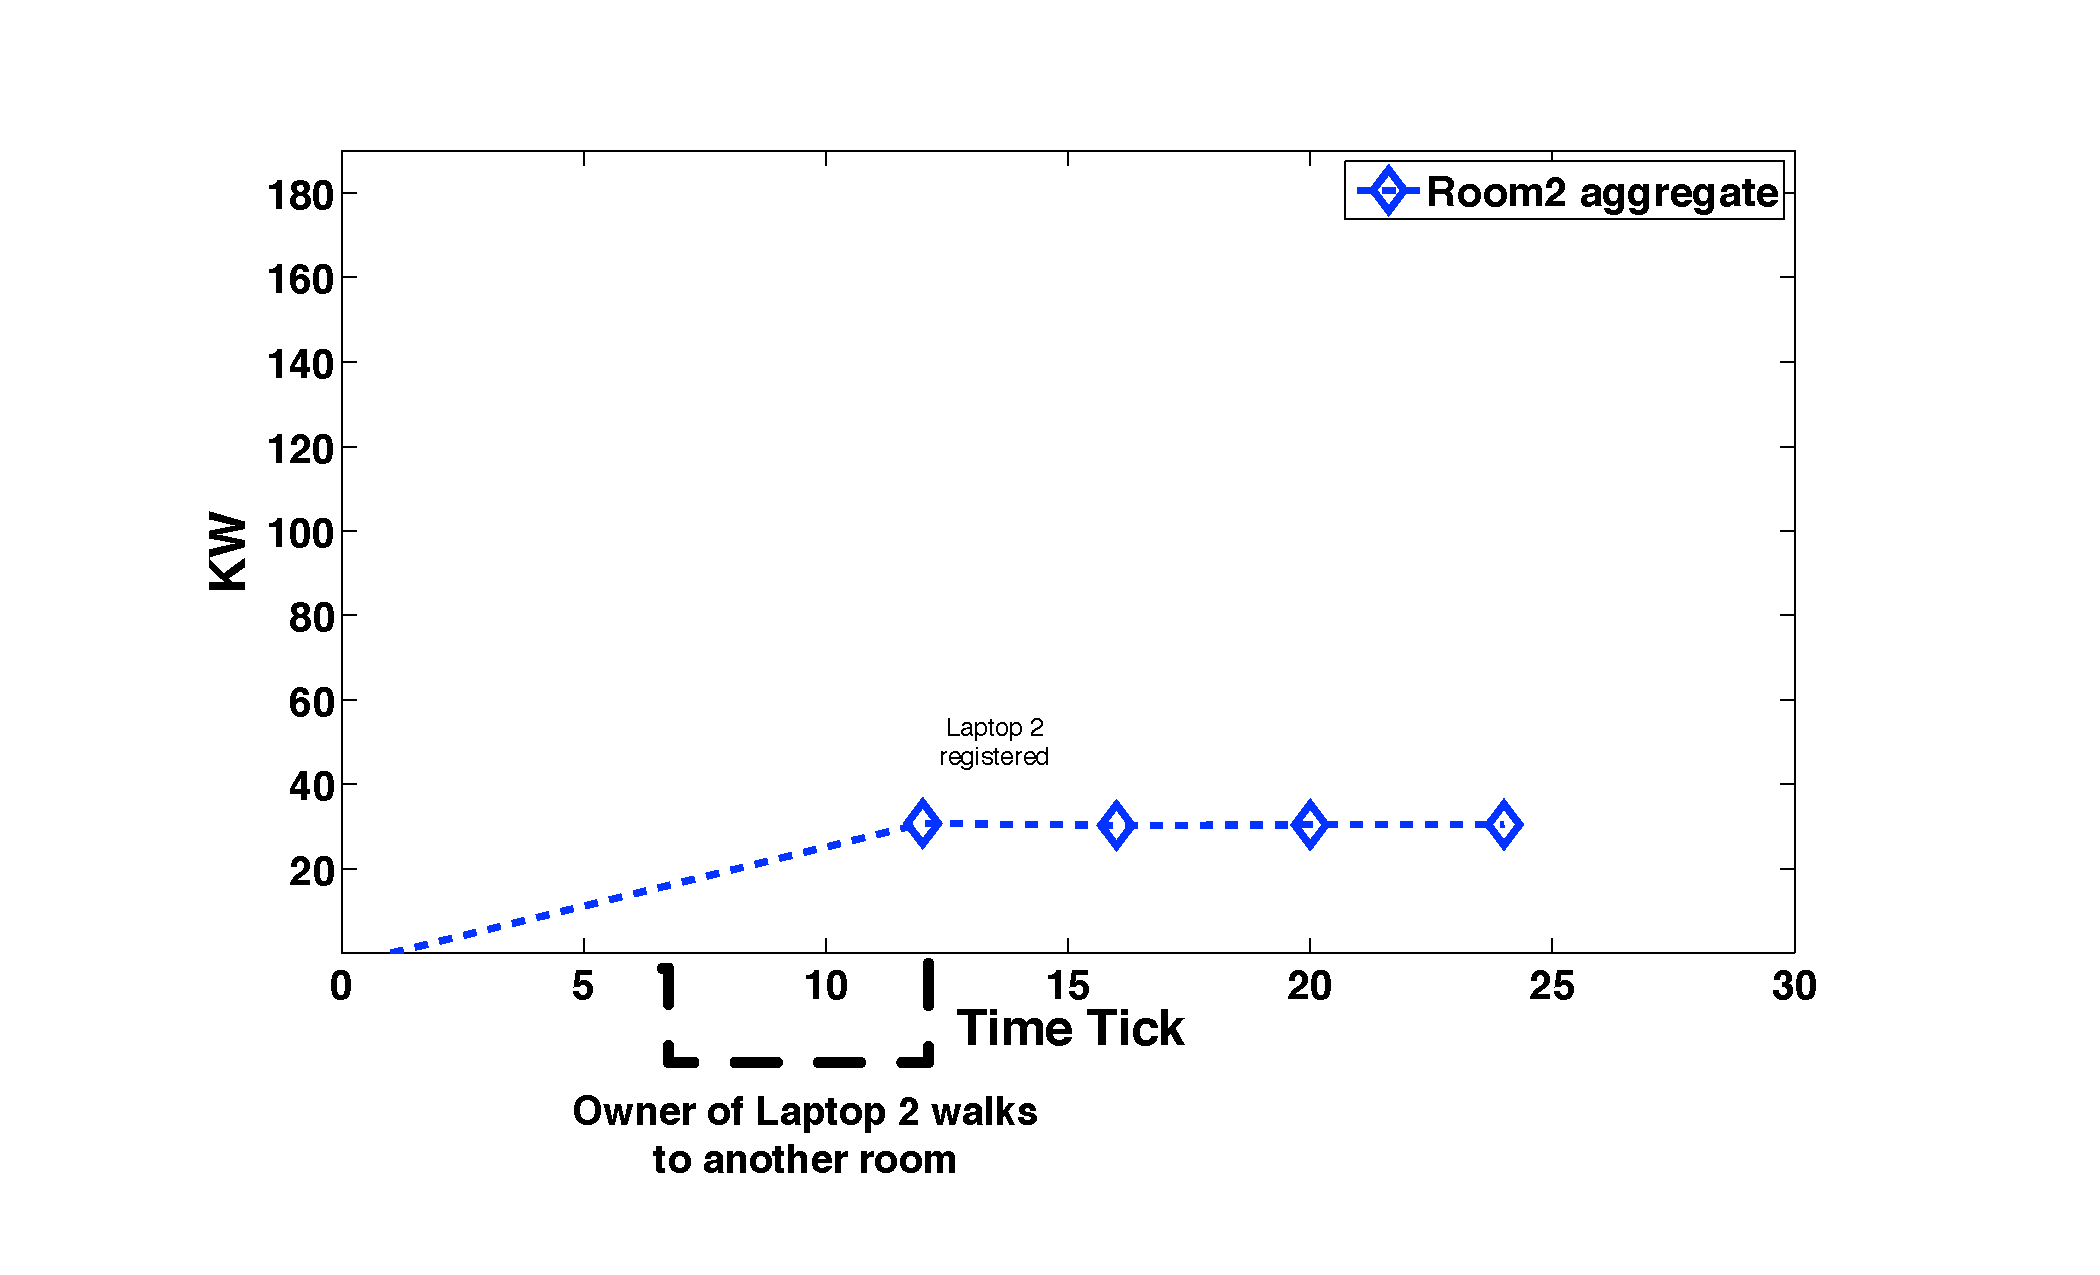
\includegraphics[scale=0.28]{figs/dynagg_scenario1_room2.pdf}
        }
\end{center}
\caption{
	The power consumes by a laptop in \emph{room 1} is shifted to \emph{room 2} a time t=7.  Notice the aggregagate drops in room 1
	while it rises in room 2.
     }%
\label{fig:multiroomagg}
\end{figure}

Figure~\ref{fig:multiroomagg} show the process of dynamic aggregation.  Notice that around tick 5 there is a drop in the total power
draw curve.  As we walk to the new location, the energy consumption remains steady, but lower in room 1 while it remains steady.
Then around tick 12, the energy consumption of the room 2 aggregate rises.  Note, the level of rise and fall of both curves is the same
30 Watts.


\begin{figure}[h!] %htbp
\centering
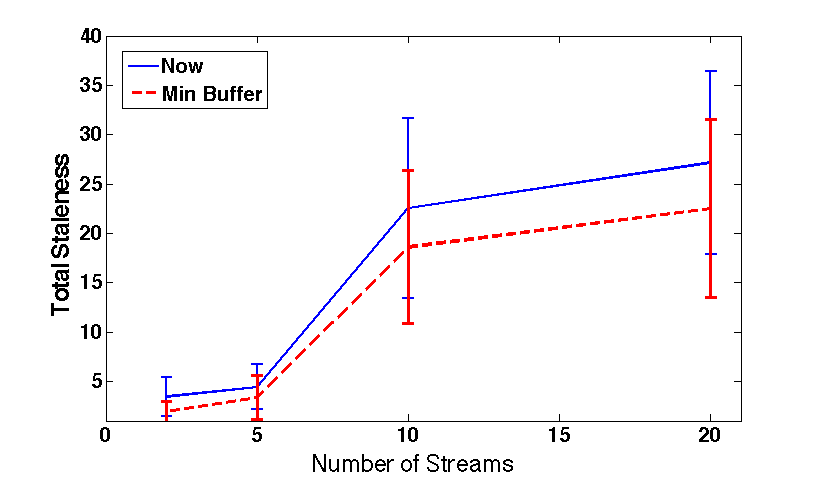
\includegraphics[width=0.75\columnwidth]{figs/staleness_vs_numstreams}
\caption{This figures shows the tradeoff between staleness and the number of streams being consumed by the job.  Note 
that out algorithm reduces the staleness of the buffer.}
\label{fig:stalevsstreams}
\end{figure}

\subsection{Maximum Freshness Methodology and Results}

We simulated the effects of the \texttt{max\_buffer} algorithm shown in algorithm~\ref{alg:min_buffer}.  We start up multiple streams and
have them feed a subscription with the algorithm option enabled.  A single run of the experiment consists of 10 runs with $k$ active streams,
where $k$ is between 1 and 20.  We let it run for some time and record the total staleness for each run, which is the sum for all data points, between
when the data point arrived and the current time.  We compare these against the default case where data is delivered as soon as at least one data point from every stream arrives.  Figure~\ref{fig:stalevsstreams} shows the returns of our experiment.

Note, the staleness increases for both cases.  The variance of both is also similar, however, the average staleness is lower 
when the \texttt{min\_buffer} algorithm is used.  It's important to note that this is always true, since the decision is explicitly
bounded by the the ``now'' case.  The algorithm chooses between ``now'' and waiting later for a better staleness calculation.

We also examine the predictability in the report rate of the job that enables this feature.  Most streams in the system report data periodically
with a very small variance around the delivery mean.  However, because the algorithm may decide that waiting is better, the delivery
period variance is larger.  Observe the effects of \texttt{min\_buffer} versus the default case.

\begin{figure}[th!] %htbp
\centering
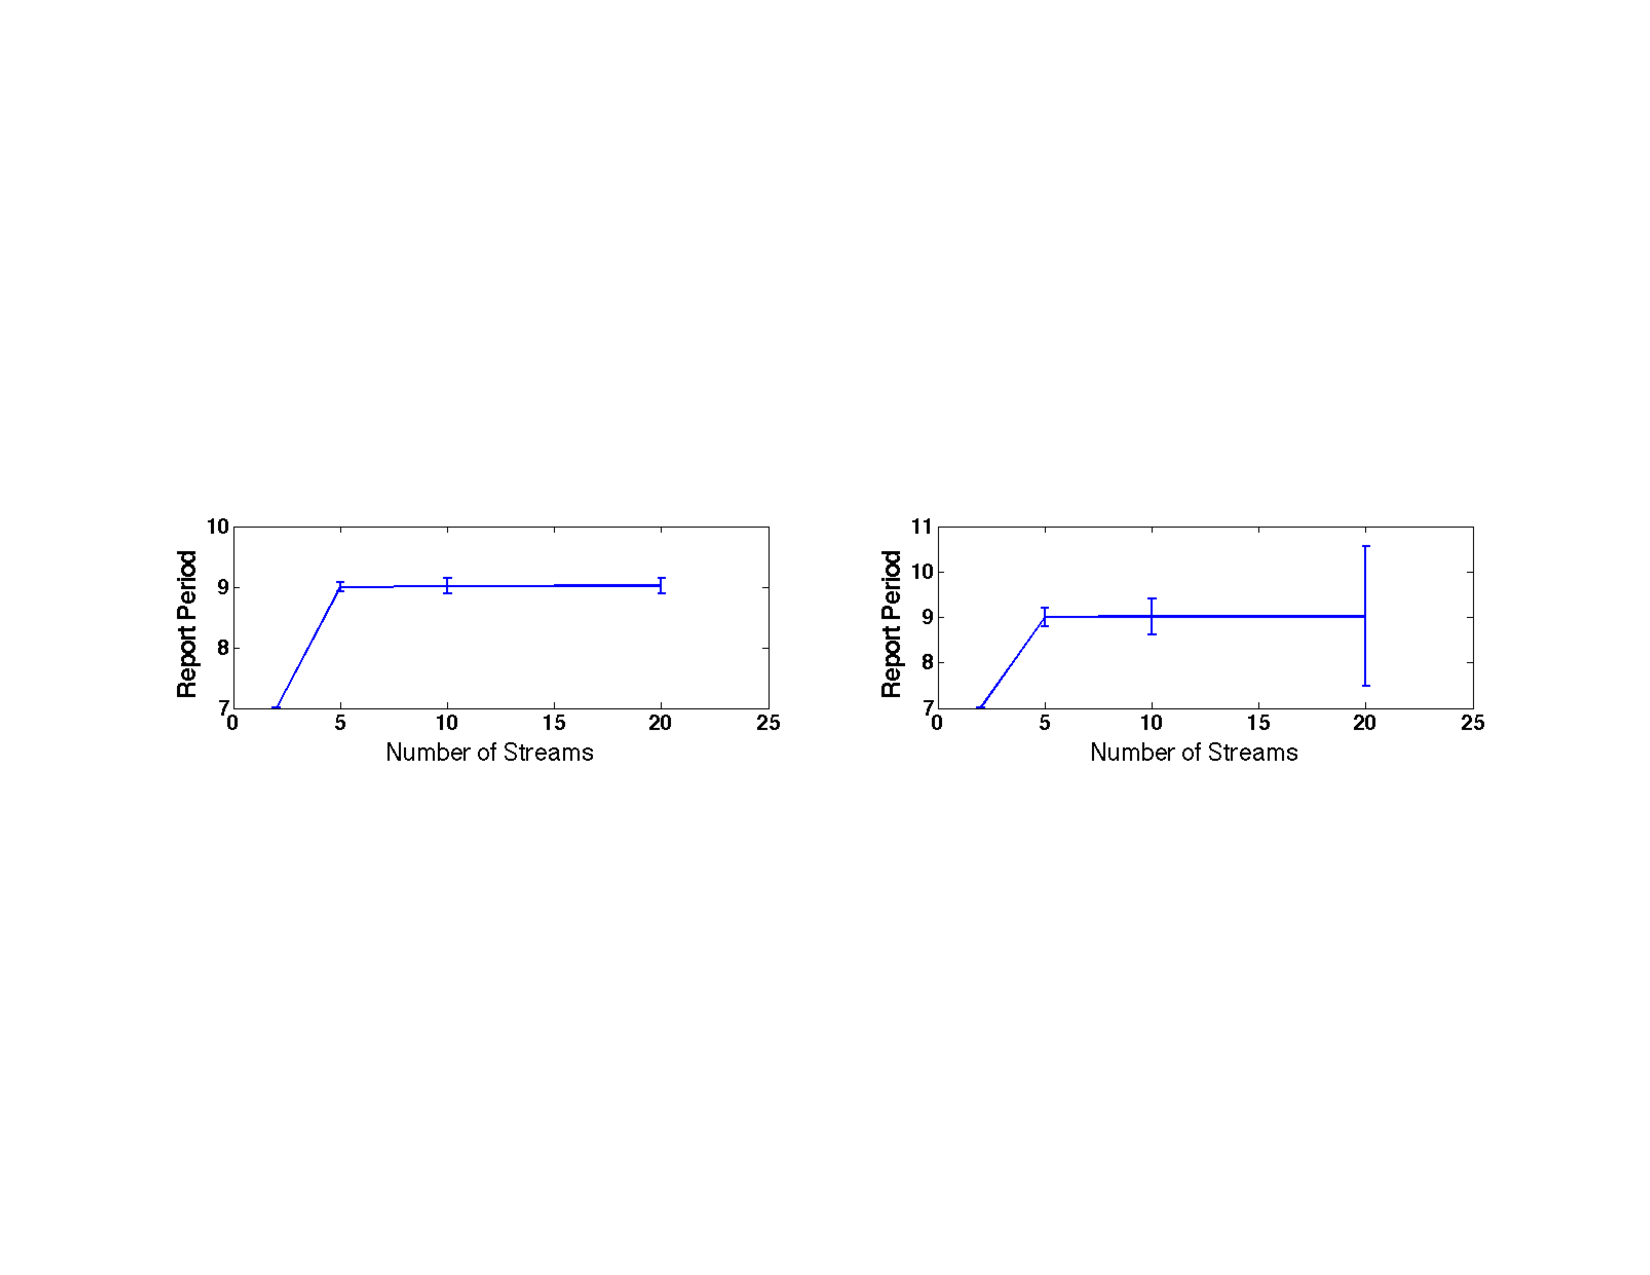
\includegraphics[width=1.0	\columnwidth]{figs/period_vs_streams}
\caption{This figures shows that the \texttt{min\_buffer} algorithm provides a similar average execution period but generally
at the cost of higher variance in delivery times.}
\label{fig:report_periods}
\end{figure}

We see that the average are practically the same, however the error bar on the graph on the right are larger.  This should be considered 
when the feature is enable.  If there is a job that consumes feeds from the output of a process that has enabled this, it should tolerate
delivery times with variable delivery rates.


